\documentclass{beamer}
\usepackage[utf8]{inputenc}
\usepackage[export]{adjustbox}
\usepackage{hyperref}
\hypersetup{
	colorlinks=true,
	urlcolor=adcorange,
	linkcolor=adcblue
}

\usetheme{Madrid}

\title{Let's make a todo list app with React Native!}
\subtitle{State manipulation!}
\author{Nathaniel Budijono}
\date{February 8, 2022}
\institute{UMN ADC}

\definecolor{adcblue}{RGB}{115,203,255}
\definecolor{adcorange}{RGB}{242,114,0}

\setbeamercolor{palette primary}{fg=white,bg=adcblue}
\setbeamercolor{palette secondary}{fg=adcorange,bg=white}
\setbeamercolor{structure}{fg=adcblue,bg=white}
\setbeamercolor{title in head/foot}{fg=adcblue,bg=white}
\setbeamercolor{date in head/foot}{fg=gray,bg=white}
\setbeamercolor{palette tertiary}{fg=white,bg=adcorange}

\begin{document}

\begin{frame}
    \titlepage
    \includegraphics[width=0.25\textwidth, right]{figs/ADC_Logo_Blue.png}
\end{frame}

\begin{frame}{Officer openings!}
	\begin{itemize}
		\item Workshop instructors
	\end{itemize}

	\bigskip

	DM us on the discord!

	\bigskip

	\href{https://z.umn.edu/ADCdiscord}{https://z.umn.edu/ADCdiscord}
\end{frame}

\begin{frame}{Guide}
	We will be following this guide: \href{https://github.com/ADC-UMN/todotorial}{https://github.com/ADC-UMN/todotorial}. Feel free to go ahead of the workshops at your own pace.
\end{frame}

\begin{frame}{What we're starting with}
	\centering
	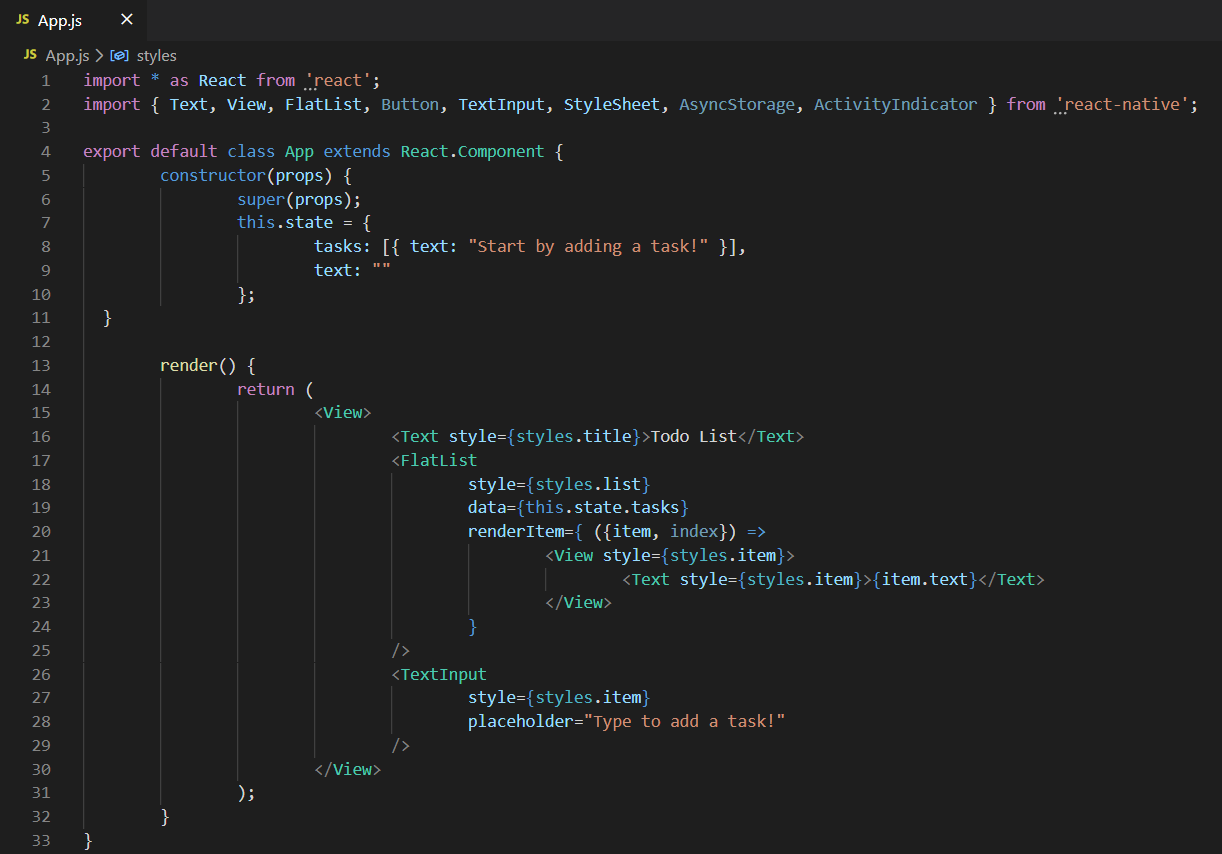
\includegraphics[width=0.9\textwidth]{figs/after-styles.png}	
\end{frame}

\begin{frame}{Goals}
	\begin{enumerate}
		\item Ability to add items \pause
		\item Ability to delete items
	\end{enumerate}
\end{frame}

\begin{frame}{Research}
	\begin{itemize}
		\item \texttt{TextInput} \href{https://reactnative.dev/docs/textinput}{https://reactnative.dev/docs/textinput}
		\begin{itemize}
			\item \texttt{onChangeText}
			\item \texttt{onSubmitEditing}
			\item \texttt{returnKeyLabel}
			\item \texttt{returnKeyType}
		\end{itemize} \pause
		\item \texttt{Button} \href{https://reactnative.dev/docs/button}{https://reactnative.dev/docs/button}
		\begin{itemize}
			\item \texttt{onPress}
		\end{itemize}
	\end{itemize}
\end{frame}

\begin{frame}{Updating the state}
	\begin{enumerate}
		\item Write \texttt{updateText()} \pause
		\item Assign the \texttt{onChangeText} prop
	\end{enumerate}
\end{frame}

\begin{frame}{Adding tasks}
	\begin{enumerate}
		\item Write \texttt{addTask()} \pause
		\item Assign the \texttt{onSubmitEditing} prop \pause
		\item Assign the \texttt{returnKeyLabel} and \texttt{returnKeyType} props
	\end{enumerate}
\end{frame}

\begin{frame}{Deleting tasks}
	\begin{enumerate}
		\item Write \texttt{deleteTask()} \pause
		\item Assign the \texttt{onPress} prop
	\end{enumerate}
\end{frame}

\end{document}